\documentclass[11pt]{article}

\usepackage{graphicx}
\usepackage{wrapfig}
\usepackage{url}
\usepackage{wrapfig}
\usepackage{color}
\usepackage{marvosym}
\usepackage{enumerate}
\usepackage{subfigure}
\usepackage{tikz}
\usepackage{amsmath}
\usepackage{amssymb}
\usepackage{hyperref}
\usepackage{epstopdf}



\oddsidemargin 0mm
\evensidemargin 5mm
\topmargin -20mm
\textheight 240mm
\textwidth 160mm



\newcommand{\vwi}{{\bf w}_i}
\newcommand{\vw}{{\bf w}}
\newcommand{\vx}{{\bf x}}
\newcommand{\vy}{{\bf y}}
\newcommand{\vh}{{\bf h}}
\newcommand{\vb}{{\bf b}}
\newcommand{\vd}{{\bf d}}
\newcommand{\vxi}{{\bf x}_i}
\newcommand{\yi}{y_i}
\newcommand{\vxj}{{\bf x}_j}
\newcommand{\vxn}{{\bf x}_n}
\newcommand{\yj}{y_j}
\newcommand{\ai}{\alpha_i}
\newcommand{\aj}{\alpha_j}
\newcommand{\W}{{\bf W}}
\newcommand{\X}{{\bf X}}
\newcommand{\Y}{{\bf Y}}
\newcommand{\vz}{{\bf z}}
\newcommand{\msigma}{{\bf \Sigma}}
\newcommand{\vmu}{{\bf \mu}}
\newcommand{\vmuk}{{\bf \mu}_k}
\newcommand{\msigmak}{{\bf \Sigma}_k}
\newcommand{\vmuj}{{\bf \mu}_j}
\newcommand{\msigmaj}{{\bf \Sigma}_j}
\newcommand{\pij}{\pi_j}
\newcommand{\pik}{\pi_k}
\newcommand{\D}{\mathcal{D}}
\newcommand{\el}{\mathcal{L}}
\newcommand{\N}{\mathcal{N}}
\newcommand{\vxij}{{\bf x}_{ij}}
\newcommand{\vt}{{\bf t}}
\newcommand{\yh}{\hat{y}}
\newcommand{\code}[1]{{\footnotesize \tt #1}}
\newcommand{\alphai}{\alpha_i}

\pagestyle{myheadings}
\markboth{Homework 4}{Fall 2015 CS 475 Machine Learning: Homework 4}


\title{CS 475 Machine Learning: Homework 4\\The EM Algorithm (and more)\\
\Large{Due: Monday November 9, 2015, 11:59pm}\\
100 Points Total \hspace{1cm} Version 1.0}
\author{}
\date{}

\begin{document}
\large
\maketitle
\thispagestyle{headings}

\vspace{-.5in}

{\bf Make sure to read from start to finish before beginning the assignment.}


\section{Programming (60 points)}
A popular type of recurrent neural network is the Boltzmann machine, the development of which goes back to the mid 1980s. Boltzmann machines
are neural networks that can learn internal representations. While learning Boltzmann machines are challenging, a common variant, the Restricted Boltzmann
Machine (RBM) allows for efficient learning algorithms. For this reason, and others, many deep networks are composed of RBMs.
A RBM is characterized by two layers: a hidden layer and an observed layer. These two layers form a bipartite graph, i.e., there are no connections within a layer.
The observed layer is the input and the learned representation is captured by the hidden layer.

In this assignment, you will implement the gradient based learning algorithm for a RBM given its training data. Since RBMs have both observed and latent variables, the EM algorithm is used for learning. In the M-step, you will use gradient based optimization to update the parameters. In the E-step, you will compute the expectations of the variables using the current model parameters. For simplicity, we will use small networks where exact inference is possible for the E-step. In practice, more complex networks require approximate inference techniques for efficient learning.

\subsection{RBM} %%%%%%%%%%%%%%%%%%%%%%%%%%%%%%%%%%%%%%%%%%%%%%%%%%%%%%%%
Consider the following RBM configuration with $n$ latent variables and $m$ observed variables, all of which are binary valued.
\begin{figure*}[h]
	\begin{center}
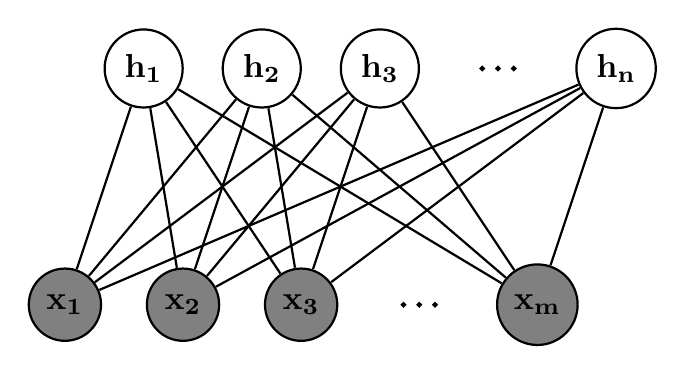
\begin{tikzpicture}[style=thick,scale=1]
\begin{scope}[shape=circle,minimum size=0.1cm]
\newcommand{\nodesizeSmall}{1.2}
\tikzstyle{every node}=[draw,fill]
\node[fill=gray,scale=\nodesizeSmall] (X_1) at (0,0) {$\mathbf{x_1}$};
\node[fill=gray,scale=\nodesizeSmall] (X_2) at (1.5,0) {$\mathbf{x_2}$};
\node[fill=gray,scale=\nodesizeSmall] (X_3) at (3,0) {$\mathbf{x_3}$};
\node[fill=gray,scale=\nodesizeSmall] (X_4) at (6,0) {$\mathbf{x_m}$};
\node[fill=none,scale=\nodesizeSmall] (X_5) at (1,3) {$\mathbf{h_1}$};
\node[fill=none,scale=\nodesizeSmall] (X_6) at (2.5,3) {$\mathbf{h_2}$};
\node[fill=none,scale=\nodesizeSmall] (X_7) at (4,3) {$\mathbf{h_3}$};
\node[fill=none,scale=\nodesizeSmall] (X_8) at (7,3) {$\mathbf{h_n}$};
\draw (5.3,3) circle (.02cm);
\draw (5.5,3) circle (.02cm);
\draw (5.7,3) circle (.02cm);
\draw (4.3,0) circle (.02cm);
\draw (4.5,0) circle (.02cm);
\draw (4.7,0) circle (.02cm);
\draw [-] (X_1) -- (X_5);
\draw [-] (X_1) -- (X_6);
\draw [-] (X_1) -- (X_7);
\draw [-] (X_1) -- (X_8);
\draw [-] (X_2) -- (X_5);
\draw [-] (X_2) -- (X_6);
\draw [-] (X_2) -- (X_7);
\draw [-] (X_2) -- (X_8);
\draw [-] (X_3) -- (X_5);
\draw [-] (X_3) -- (X_6);
\draw [-] (X_3) -- (X_7);
\draw [-] (X_3) -- (X_8);
\draw [-] (X_4) -- (X_5);
\draw [-] (X_4) -- (X_6);
\draw [-] (X_4) -- (X_7);
\draw [-] (X_4) -- (X_8);
\end{scope}
\end{tikzpicture}
		
			\label{fig:rbm}
		\end{center}
\end{figure*}

Probability in RBM models is often expressed as ``energy'', where maximizing the probability means minimizing the energy. The joint probability
distribution for the variables in this RBM is given by:
\begin{equation}
\label{eq:joint}
p(\vx, \vh;\theta) = \frac{1}{Z} \exp\{-E_\theta(\vx, \vh)\}
\end{equation}
where $E_\theta(\vx, \vh)$ is the energy function and $Z$ is the partition function that normalizes the distribution. In this notation, $\vh$ are the hidden variables and $\vx$ are the observed variables. The energy function is defined as:
\begin{equation}
E_\theta(\vx, \vh) = -\vx^T \mathbf{W}\vh - \vb^T\vx - \vd^T\vh
\end{equation}
We define the model parameters as $\theta:=\{\W,\vb,\vd\}$, where $\mathbf{W} = (w_{i,j})$ is a matrix of weights associated with the connection between the visible unit $x_i$ and the hidden unit $h_j$.
$\vb$ and $\vd$ are vectors, where the $i$th position of $\vb$ ($b_i$) and and the $j$th position of $\vd$ ($d_j$) correspond
to the bias parameters for the observed variable $x_i$ and the latent variable $h_j$  respectively.

The partition function $Z$ is used to normalize the energy function to obtain a probability distribution:
\begin{equation}
Z = \sum_{(\vx,\vh)} \exp\{-E_\theta(\vx, \vh)\}
\end{equation}
which sums over all possible combinations of the vectors $\vx$ and $\vh$.

Using the conditional independence assumptions inherent in this model, we obtain the following probabilities:
\begin{equation}
p(\vx|\vh;\theta) = \prod_{i=1}^{m} p(x_i|\vh;\theta)
\end{equation}
\begin{equation}
\label{eq:cond}
p(\vh|\vx;\theta) = \prod_{j=1}^{n} p(h_j|\vx;\theta)
\end{equation}

The conditional probability of a single variable (e.g., $p(x_i=1|\vh;\theta)$) is represented using a sigmoid activation function $\sigma(z)$:
\begin{equation}
\label{eq:phx}
p(h_j=1|\vx;\theta) = \sigma(\vx^T\W_{-,j} + d_j)
\end{equation}

\begin{equation}
\label{eq:pxh}
p(x_i=1|\vh;\theta) = \sigma(\vh^T\W_{i,-}^T + b_i)
\end{equation}
where $\W_{-,j}$ is the $j$th column of $\W$, $\W_{i,-}$ is the $i$th row of $\W$, and $\sigma(z)$ is defined as:
\begin{equation}
\sigma(z) = \frac{1}{1+\exp(-z)}
\end{equation}

The likelihood of a single example $\vx$ is given by:
\begin{equation}
p(\vx;\theta) = \sum_{\vh} \frac{1}{Z} \exp\{-E_\theta(\vx, \vh)\}
\end{equation}

With $T$ training examples, the log likelihood is given by:
\begin{equation}
\sum_{t=1}^T \log p(\vx^{(t)};\theta) = \sum_{t=1}^T \log \sum_{\vh} \frac{1}{Z} \exp\{-E_\theta(\vx^{(t)}, \vh)\}
\end{equation}

Gradient-based optimization requires the gradients of the parameters, which for the RBM is given by:
\begin{eqnarray}
\nonumber
\frac{\partial}{\partial \W_{i,j}}\sum_{t=1}^T \log p(\vx^{(t)};\theta) &=& \frac{\partial}{\partial \W_{i,j}}\sum_{t=1}^T \log \frac{\sum_{\vh}\exp\{-E_\theta(\vx^{(t)},\vh)\}}{\sum_{(\vx,\vh)}\exp\{-E_\theta(\vx,\vh)\}} \\\nonumber
&=& \sum_{t=1}^T \frac{\partial}{\partial \W_{i,j}} \log \sum_{\vh}\exp\{-E_\theta(\vx^{(t)},\vh)\} - \sum_{t=1}^T \frac{\partial}{\partial \W_{i,j}} \log\sum_{(\vx,\vh)}\exp\{-E_\theta(\vx,\vh)\}\\\nonumber
&=& \sum_{t=1}^T \frac{\sum_{\vh} \exp\{-E_\theta(\vx^{(t)},\vh)\}(-\frac{\partial}{\partial \W_{i,j}}E_\theta(\vx^{(t)},\vh))}{\sum_{\vh} \exp\{-E_\theta(\vx^{(t)},\vh)\}}\\\nonumber
&&-\sum_{t=1}^T \frac{\sum_{(\vx,\vh)} \exp\{-E_\theta(\vx,\vh)\}(-\frac{\partial}{\partial \W_{i,j}}E_\theta(\vx,\vh))}{\sum_{(\vx,\vh)} \exp\{-E_\theta(\vx,\vh)\}} \\\nonumber
&=& -\sum_{t=1}^T \mathbb{E}_{p(\vh|\vx^{(t)};\theta)}\left[\frac{\partial}{\partial \W_{i,j}}E_\theta(\vx^{(t)},\vh)\right]+ \sum_{t=1}^T \mathbb{E}_{p(\vx,\vh;\theta)}\left[\frac{\partial}{\partial \W_{i,j}}E_\theta(\vx,\vh)\right] \\ \label{eq:der1}
&=& -\sum_{t=1}^T \mathbb{E}_{p(\vh|\vx^{(t)};\theta)}\left[-x_i^{(t)}h_j\right]+ \sum_{t=1}^T \mathbb{E}_{p(\vx,\vh;\theta)}\left[-x_ih_j\right] \\ \label{eq:der2}
\frac{\partial}{\partial \vb_i} \sum_{t=1}^T \log p(\vx^{(t)};\theta) &=& -\sum_{t=1}^T \mathbb{E}_{p(\vh|\vx^{(t)};\theta)}\left[-x_i^{(t)}\right]+ \sum_{t=1}^T \mathbb{E}_{p(\vx,\vh;\theta)}\left[-x_i\right] \\\label{eq:der3}
\frac{\partial}{\partial \vd_j} \sum_{t=1}^T \log p(\vx^{(t)};\theta) &=& -\sum_{t=1}^T \mathbb{E}_{p(\vh|\vx^{(t)};\theta)}\left[-h_j\right]+ \sum_{t=1}^T \mathbb{E}_{p(\vx,\vh;\theta)}\left[-h_j\right]
\end{eqnarray}
where we have the expectations with respect to $p(\vh|\vx^{(t)};\theta)$, and  $p(\vx,\vh;\theta)$. Intuitively, the gradient acts
to move the two expectations close to each other until the gradient is 0, at which point the gradient of the energy functions have equal expectations with $\vx$ sampled from the training distribution or with $\vx$ sampled from the model. In other words, the distribution from the model and the training data agree with each other.

The M-step is comprised of updating the model parameters using the gradients defined in Eq.~(\ref{eq:der1},\ref{eq:der2},\ref{eq:der3}). As is typical in the EM algorithm, this M-step depends on computing the expectation of the hidden variables according to the model parameters $p(\vh|\vx^{(t)};\theta)$ and the joint of the hidden and observed variables $p(\vx,\vh;\theta)$. Note that we need to compute these distributions for all possible combinations of $\vx,\vh$ given the current estimate of the parameters $\theta$. Obviously for large networks, we could never sum over all possible combinations. However, in this homework we will restrict ourselves to small networks (i.e. with very few binary-valued nodes) where these summations are tractable using Eq.~(\ref{eq:joint}) and Bayes rules.

Note that before computing the expectations, we can first marginalize over variables that do not appear inside the expectations. For example, you can replace $p(\vh|\vx^{(t)})$ with $p(h_j|\vx^{(t)};\theta)$, and $p(\vx,\vh;\theta)$ with $p(x_i,h_j;\theta)$ in Eq.~(\ref{eq:der1}) since the functions inside the expectations only involve $x_i$ and $h_j$.

To give you a specific example, Eq.~(\ref{eq:der1}) would be derived as:
\begin{eqnarray}
\nonumber
&&-\sum_{t=1}^T \mathbb{E}_{p(\vh|\vx^{(t)};\theta)}\left[-x_i^{(t)}h_j\right]+\sum_{t=1}^T \mathbb{E}_{p(\vx,\vh;\theta)}\left[-x_ih_j\right] \\
\label{eq:der4}
&=&-\sum_{t=1}^T \mathbb{E}_{p(h_j|\vx^{(t)};\theta)}\left[-x_i^{(t)}h_j\right]+T\cdot \mathbb{E}_{p(x_i,h_j;\theta)}\left[-x_ih_j\right] \\
\label{eq:der5}
&=&-\sum_{t=1}^T \sum_{h_j}{p(h_j|\vx^{(t)};\theta)}\left(-x_i^{(t)}h_j\right)+T\cdot \sum_{x_i,h_j}{p(x_i,h_j;\theta)}\left(-x_ih_j\right) \\
\label{eq:der6}
&=&-\sum_{t=1}^T p(h_j=1|\vx^{(t)};\theta)\left(-x_i^{(t)}\right)-T \cdot p(x_i=1,h_j=1;\theta) \\
\label{eq:der7}
&=& -\sum_{t=1}^T \sigma(\vx^{(t)T}\W_{-,j} + d_j)\left(-x_i^{(t)}\right)-T \cdot\sum_{\vx_{-i},\vh_{-j}}p(\vx_{-i},\vh_{-j},x_i=1,h_j=1;\theta)
\end{eqnarray}
where we denote all variables in $\vx$ (and $\vh$) except $x_i$ (and $h_j$) as $\vx_{-i}$ (and $\vh_{-j}$) in Eq.~(\ref{eq:der7}), and the expectations in Eq.~(\ref{eq:der4}) are expanded as in Eq.~(\ref{eq:der5}) by definition. E.g., $\mathbb{E}_{p(h_j|\vx^{(t)};\theta)}\left[-x_i^{(t)}h_j\right]$ is the expected value of $-x_i^{(t)}h_j$ when $h_j \sim p(h_j|\vx^{(t)};\theta)$.


\subsection{Initialization}
\label{sec:init}
We need to randomly initialize the parameters $\theta^{(0)}=\{\W^{(0)},\vb^{(0)},\vd^{(0)}\}$. To ensure that everyone gets the same values of all the parameters, you must use the following procedure {\em exactly}. 
\begin{eqnarray}
\W^{(0)}_{i,j}=\left\{ \begin{array}{ll}
1 & \textrm{if $j$ is even} \\
0 & \textrm{otherwise}
\end{array} \right.
\vb^{(0)}_{i}=\left\{ \begin{array}{ll}
1 & \textrm{if $i$ is even} \\
0 & \textrm{otherwise}
\end{array} \right.
\vd^{(0)}_{j}=\left\{ \begin{array}{ll}
1 & \textrm{if $j$ is even} \\
0 & \textrm{otherwise}
\end{array} \right.
\end{eqnarray}
%Create a \code{java.util.Random} object \code{rnd} with a seed of 0. Only use this object for initialization. You will start by initialize the values for the matrix $\W^{(0)}$. Sample positions of the matrix in increasing order, starting from the $(0,0)$-th position, then next the $(0,1)$-th position,..., and finally the $(m-1,n-1)$-th pposition. Each value should be generated with a single call to the \code{nextDouble()} method on the \code{Random} object, then scaled by 2, finally subtracted by 1, (\code{rnd.nextDouble()*2-1} which makes the value to be within the range $[-1,1]$). You will then repeat this for the initialization procedure for the vectors $\vb^{(0)}$ and $\vd^{(0)}$. Each iteration should proceed in this fashion.
\subsection{The Framework of learning RBM}
Using the above derivations, learning an RBM network proceeds as follows.
\begin{enumerate}
\item Set learning rate $\eta$ and number of iterations $K$.
\item Initialize all the parameters $\theta^{(0)}=\{\W^{(0)},\vb^{(0)},\vd^{(0)}\}$ according to Sec.~\ref{sec:init}.
\item E-Step: compute the probabilities $p(\vh|\vx^{(t)};\theta)$ and $p(\vx,\vh;\theta)$ based on current model parameters.
\item M-Step: update parameters $\theta^{(k)}=\theta^{(k-1)}+\eta \frac{\partial}{\partial \theta^{(k-1)}} \sum_{t=1}^T \log p(\vx^{(t)};\theta^{(k-1)})$ using Eq.~(\ref{eq:der1},\ref{eq:der2},\ref{eq:der3}).
\item Repeat E-Step and M-Step for $K$ iterations.
\end{enumerate}

\subsection{Implementation} %%%%%%%%%%%%%%%%%%%%%%%%%%%%%%%%%%%%%%%%%%%%%%%%%%%%%%%%%%%%%%
\textbf{IMPORTANT}: You are {\em only} allowed to {\em add} your own code in \code{cs475.RBM.RBMEnergy}. {\em Do not} delete any existing code.

We have provided you 3 samples of the data file, \code{RBM\_data.txt}. The format is \code{"m n T"} on the first line, where $m$ is the number of  input(visible) nodes $\vx$, $n$ is the number of the hidden nodes $\vh$ and $T$ is the number of training examples, followed by $T$ lines of training examples, each of which is an observation of length $m$.

You will be able to get the values for $m$ and $n$ by calling the following functions in \code{cs475.RBM.RBMParameters}:
\begin{footnotesize}
\begin{verbatim}
    public int numVisibleNodes()   // returns m
    public int numHiddenNodes()  // returns n
    public int numExamples()  // returns T
\end{verbatim}
\end{footnotesize}
We have also provided functions in \code{cs475.RBM.RBMParameters} that give you the values of the visible nodes, the bias parameters and the weights, and functions that update these parameters,
\begin{footnotesize}
\begin{verbatim}
    public double getExample(int t, int i)//returns the value of node x_i for example t
    public double getVisibleBias(int i)  // returns the bias for node x_i
    public double getHiddenBias(int i)  // returns the bias for node h_i
    public double getWeight(int i, int j) // returns the weight(i,j)
    public boolean setVisibleBias(int i, double val)  // sets the bias for node x_i
    public boolean setHiddenBias(int i, double val)  // sets the bias for node h_i
    public boolean setWeight(int i, int j, double val) // sets the weight W_(i,j)
\end{verbatim}
\end{footnotesize}

\subsubsection{Command Line Arguments}
We have already added 3 command line options in \code{cs475.RBM.RBMTester} for you.
\begin{footnotesize}
\begin{verbatim}
    registerOption("data", "String", true, "The data to use.");
    registerOption("gd_eta", "double", true, "The constant scalar for learning rate. default: 0.1");
    registerOption("gd_iterations", "int", true, "The number of iterations.default: 20");
\end{verbatim}
\end{footnotesize}

\subsubsection{What You Need to Implement} %%%%%%%%%%%%%%%%%%%%%%%%%%%%%%%%%%%%%%%%%%%%%%%%%%%%
We have provided you with the class \code{cs475.RBM.RBMEnergy} with one method left blank that you will need to implement:
\begin{footnotesize}
\begin{verbatim}
public class RBMEnergy {
    	public double learning() {
    		
    		// TODO: Add code here
    		
    	}
}

\end{verbatim}
\end{footnotesize}

\subsection{How We Will Run Your Code} %%%%%%%%%%%%%%%%%%%%%%%%%%%%%%%%%%%%%%%%%%%%%%%%%%%%
We will run your code using the data file and the following command line arguments:
\begin{footnotesize}
\begin{verbatim}
    java cs475.RBM.RBMTester -data RBMData.txt  \
    -gd_iterations K -gd_eta eta
\end{verbatim}
\end{footnotesize}
Note: we may use data files with different values of $m$ and $n$, so make sure your code works for any reasonable input.\\
\\
Your output should just be the results of the print statements in the code given. {\bf Do not print anything else in the version you hand in.}


\section{Analytical Questions (40 points)}

\paragraph{1. Overfitting in Clustering (10 points)}

Given the data set $x_1,...,x_n$, we want to do clustering by the K-means algorithm. The K-means algorithm aims to partition the $n$ observations into $k$ sets ($k < n$) $S = \{S_1, S_2, ... , S_k\}$ so as to minimize the within-cluster sum of squares
\begin{eqnarray*}
\mathop{\textrm{min}}_{S=\{S_1,...,S_k\}}\sum_{j=1}^k\sum_{x_i\in S_j}\|x_j-\mu_j\|_2^2
\end{eqnarray*}
where $\mu_j$ is the mean of points in $S_j$.

\begin{enumerate}[(a)]
\item Prove that the objective value does not increase in each iteration of the K-means algorithm. 
\item Let $\gamma_k$ denote the global optimal objective value, prove $\gamma_k$ is non-increasing in $k$.
\end{enumerate}



\paragraph{2. Curse-of-dimensionality (10 points)}
In this problem, we study why $K$-NN could fail in high dimensions by means of a very simple example. Consider a sphere of radius $r$ in $d$-dimensions together with a concentric hypercube of side $2r$. The sphere touches the hypercube at the center of each of its sides.

\begin{enumerate}[(a)]
\item $V_c$ is the volume of the cube and $V_s$ is the volume of the sphere, where the volume of a $d$-dimensional sphere with radius $r$ is given as 
\begin{eqnarray}
V_s = \frac{r^d\sqrt{\pi}^d}{\Gamma(d/2+1)}, \nonumber
\end{eqnarray}
where $\Gamma(z)=\int_0^{\infty}t^{z-1}e^{-t}\textrm{d}t$.  Note that $\Gamma(z) = (z-1)!$ (the factorial of $z-1$) if $z$ is a positive integer.  Please show that: 
\begin{eqnarray}
\lim_{d\rightarrow\infty}\frac{V_s}{V_c} = 0
\label{CoD}
\end{eqnarray}

Note that this relies on algebra and will not require any complex calculus (just some basic facts on limits). You may find the following limit useful:
\begin{eqnarray}
\lim_{z\rightarrow\infty}\frac{\Gamma(z+1)}{\sqrt{2\pi z}e^{-z}z^z}=1 \nonumber
\end{eqnarray}

\item What is the connection between \eqref{CoD} and the curse of dimensionality?
\end{enumerate}



\paragraph{3. Semi-supervised EM algorithm (10 points)}
Suppose that some of your observed data are labelled. You have $x_1,...,x_n\in\mathbb{R}^{d}$ and $x_{n+1},...,x_{n+m}$. Meanwhile, you also know the labels corresponding to $x_{n+1},...,x_{n+m}$, i.e., $y_{n+1},...,y_{n+m}\in\{1,...,K\}$, where K is the number of clusters. Please design a Gaussian Mixture Model-based EM algorithm to cluster the data. [Hint: For $x_{n+1},...,x_{n+m}$, the corresponding labels are no longer missing values]
\begin{enumerate}[(a)]
\item Write the new likelihood objective for this new algorithm.
\item Write the new update rules in each iteration.
\end{enumerate}

\paragraph{4. Modified EM (10 points)}
The EM algorithm we learned about in class is just one of several different general EM algorithms, all with similar goals and structures.  In this problem we will consider an alternative EM algorithm which modifies the M-step. Instead of maximizing $\mathcal{L}(q,\theta)$ with respect to $\theta$, the algorithm selects a single parameters $\theta_i \in \theta$ and modifies
it to increase $\mathcal{L}(q,\theta)$.

\begin{enumerate}[(a)]
\item Will this new EM algorithm yield the same solution as the normal EM algorithm?
\item Will this new EM algorithm converge (assuming lack of singularities)? If yes, then prove convergence. If no, then give a counterexample illustrating why not.
\end{enumerate}



\section{What to Submit}
In each assignment you will submit two things.
\begin{enumerate}
\item {\bf Code:} Your code as a zip file named {\tt library.zip}. {\bf You must submit source code (.java files)}. We will run your code using the exact command lines described above, so make sure it works ahead of time. Remember to submit all of the source code, including what we have provided to you.
\item {\bf Writeup:} Your writeup as a {\bf PDF file} (compiled from latex) containing answers to the analytical questions asked in the assignment. Make sure to include your name in the writeup PDF and use the provided latex template for your answers.
\end{enumerate}
Make sure you name each of the files exactly as specified (library.zip and writeup.pdf).

To submit your assignment, visit the ``Homework'' section of the website (\href{http://www.cs475.org/}{http://www.cs475.org/}.)

\section{Questions?}
Remember to submit questions about the assignment to the appropriate group on the class discussion board: \href{http://bb.cs475.org/}{http://bb.cs475.org}.


\end{document}
